\documentclass[tikz,border=5mm]{standalone}
\usepackage{pgfplots}
\usepackage{amsmath}
\pgfplotsset{compat=1.18}

\definecolor{lineblue}{RGB}{0, 0, 128}
\definecolor{linered}{RGB}{128, 0, 0}
\definecolor{linegreen}{RGB}{0, 100, 0}
\definecolor{areayellow}{RGB}{255, 235, 140}
\definecolor{solidred}{RGB}{214, 24, 66}

\begin{document}
	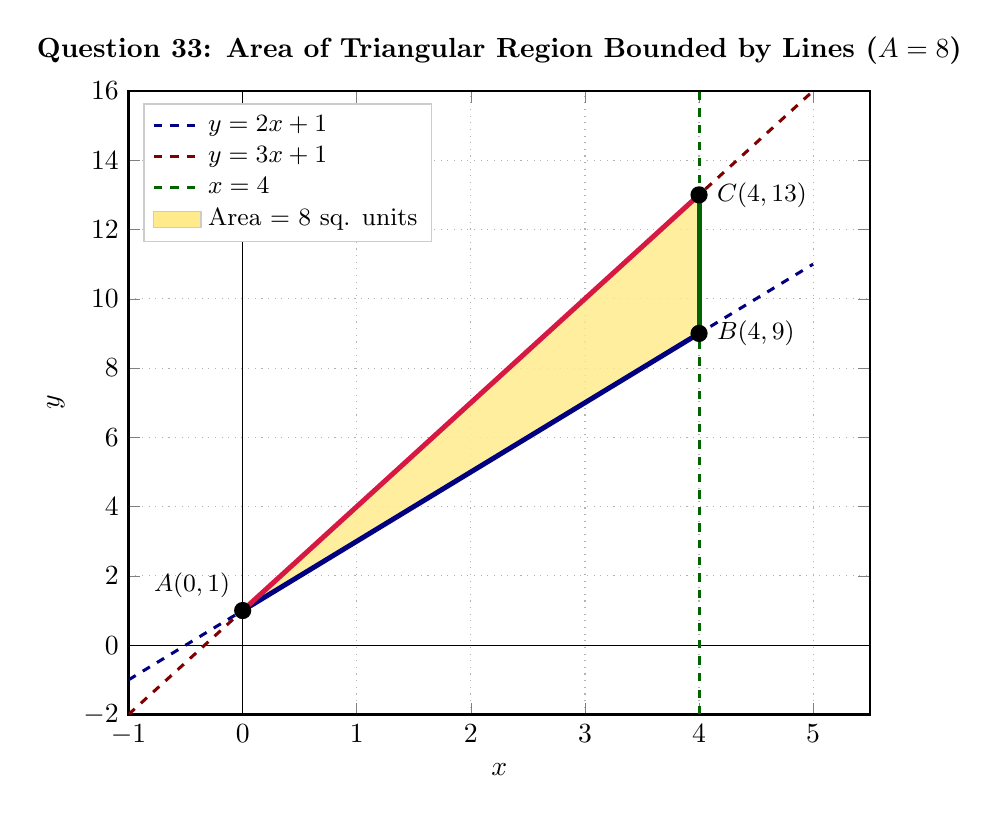
\begin{tikzpicture}
		\begin{axis}[
			width=11cm, height=9.5cm,
			title={\textbf{Question 33: Area of Triangular Region Bounded by Lines ($A = 8$)}},
			xlabel={$x$}, ylabel={$y$},
			xmin=-1, xmax=5.5,
			ymin=-2, ymax=16,
			xtick={-1, 0, 1, 2, 3, 4, 5},
			ytick={-2, 0, 2, 4, 6, 8, 10, 12, 14, 16},
			grid=both,
			grid style={dotted, gray!60},
			axis line style={black, thick},
			legend cell align={left},
			legend style={at={(0.02,0.98)}, anchor=north west, font=\small, draw=gray!40}
			]
			% Origin axis lines
			\draw[black, thin] (axis cs:0,-2) -- (axis cs:0,16);
			\draw[black, thin] (axis cs:-1,0) -- (axis cs:5.5,0);
			
			% Shaded Triangular Area
			\fill[fill=areayellow, opacity=0.85] (axis cs:0,1) -- (axis cs:4,9) -- (axis cs:4,13) -- cycle;
			
			% Extended dashed lines
			\addplot[lineblue, dashed, line width=1.1pt, domain=-1:5] {2*x + 1};
			\addlegendentry{$y = 2x + 1$}
			
			\addplot[linered, dashed, line width=1.1pt, domain=-1:5] {3*x + 1};
			\addlegendentry{$y = 3x + 1$}
			
			\addplot[linegreen, dashed, line width=1.1pt] coordinates {(4,-2) (4,16)};
			\addlegendentry{$x = 4$}
			
			% Area legend entry
			\addlegendimage{area legend, fill=areayellow, draw=none}
			\addlegendentry{Area = 8 sq. units}
			
			% Solid boundary segments of the triangle
			\draw[lineblue, line width=1.8pt] (axis cs:0,1) -- (axis cs:4,9);
			\draw[solidred, line width=1.8pt] (axis cs:0,1) -- (axis cs:4,13);
			\draw[linegreen, line width=1.8pt] (axis cs:4,9) -- (axis cs:4,13);
			
			% Vertices and labels
			\node[circle, fill=black, inner sep=2.2pt] at (axis cs:0,1) {};
			\node[above left=1pt, font=\small] at (axis cs:0,1) {$A(0, 1)$};
			
			\node[circle, fill=black, inner sep=2.2pt] at (axis cs:4,9) {};
			\node[right=3pt, font=\small] at (axis cs:4,9) {$B(4, 9)$};
			
			\node[circle, fill=black, inner sep=2.2pt] at (axis cs:4,13) {};
			\node[right=3pt, font=\small] at (axis cs:4,13) {$C(4, 13)$};
		\end{axis}
	\end{tikzpicture}
\end{document}